\newgeometry{
    top = 1.25cm,
    bottom = 2.0cm,
    left = 1.3cm,
    right = 1.3cm}
\noindent\textbf{Ответы, указания, решения}\\
\rule{12cm}{0.4pt}
\begin{multicols}{2}
    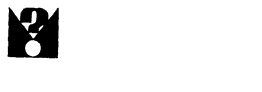
\includegraphics{image.png}
    \subsubsection*{Где расположено основание высоты?}
    З а д а ч и (мы приводим номер правильного ответа, а вслед за ним -- указание).\\
    1а---3 (основание должно быть равноудалённым от вершин основания;\\
    1б---3 (по той же причине, что 1а).\\
    1в---5 (основание должно быть равноудалено от прямых $AB$, $BC$, $AC$)\\
    1г---2 (достаточно показать, что основание высоты O принадлежит одной из высот треугольника, скажем $CH$), но\\\break
    $(SC)\perp(SA)$, $(SC)\perp(SB) \Rightarrow$\\
    \mbox{}\hfill $\Rightarrow (SC)\perp(ASB)\Rightarrow(SC)\perp(AB);$\\
    $(AB)\perp(SC)$, $(AB)\perp(SO)\Rightarrow(AB)\perp$\\
    \mbox{}\hfill $\perp(SOC)\Rightarrow(AB)\perp(CO)\Rightarrow O \in(CH)$.\\\break
    1д---2 (решение аналогично 1г)\\
    1е---6 (покажите, что $\widehat{BAC}=\widehat{BSC}=90^{\circ}$, и воспользуйтесь 1а)\\
    1ж---7 ($(AC)\perp(BC)$, $(AC)\perp(BC)\Rightarrow(AC)\perp$\\
    $\perp(BSC)\Rightarrow(ABC)\perp(BSC)\Rightarrow(SO)\subset(BSC)\Rightarrow$\\
    $\Rightarrow O \in (BC))$\\
    1з---1 (см. <<Геометрия 9---10>> \S 22).\\
    2---3 (ср. 1а).\\
    3---2 (основание высоты --- центр окружности, описанной вокруг $ABCD$).\\\break
    У п р а ж н е н и я\\
    \textbf{1.} $\frac{3\sqrt{6}}{2}a^2$. (Основание высоты --- центр окружности, вписанной в трапецию)\\
    \textbf{2.} $\frac{1}{2}$, если $a=b$.\\
    \{$\frac{b}{a+b}$, $\frac{b}{a-b}$\}, если $a>b$,\\
    \{$\frac{a}{a+b}$, $\frac{a}{a-b}$\}, если $a<b$.\\
    (Покажите, что $O \in (AC)$; далее, при $a>b$, разберите два случая: $O \in [AC]$ и $C \in [AO]$.)\\
    \textbf{3.} $\frac{c^3}{36}(\sin 2\alpha)\tan\beta$ (Примените задачу 1з.)\\
    \textbf{4.} $\frac{\sqrt{2}}{2}b^3$. (Основание равноудалённой вершины --- центр квадрата)\\
    \textbf{5.} (См. <<Квант>>, 1978, № 6, c. 93)
    \subsubsection*{Фотоаппарат на вступительных экзаменах}
    \textbf{1.} $|\overset{\rightarrow}{v}|=\frac{\delta d}{F\tau}=10m/s$.\\
    \textbf{2.} $\frac{F_2}{F_1}=1+\frac{h(d-F)}{F^2}=5.5$\\
    \textbf{3.} $d_2'=\frac{d_1d_2d_1'}{d_1'(d_1+d_2)-d_1d_2}\rightarrow\infty$, то есть дальняя граница глубины резкости бесконечно удалена.\\
    \subsubsection*{Московский государственный университет им. М. В. Ломоносова}
    \subsubsection*{Ф и з и к а\\ Физический факультет}
    \textbf{1.} $A=mg(H - 512R)=2\cdot 10^{-2}$ Дж.\\
    \textbf{2.} $V_2=l_2\sqrt{\frac{2g(1-\cos\alpha)(m_2l_2-m_1l_1)}{m_1l_1^2+m_2l_2^2}}$, если в положении устойчивого равновесия масса $m_1$ находится выше оси вращения, и\\ 
    $V_2=l_2\sqrt{\frac{2g(1+\cos\alpha)(m_1l_1-m_2l_2)}{m_1l_1^2+m_2l_2^2}}$, если в положении устойчивого равновесия масса $m_1$ находится ниже оси вражения.\\
    \textbf{3.} $|\overset{\rightarrow}{a}|=g(\sin\alpha-\frac{(k_1m_1+k_2m_2\cos\alpha)}{m_1+m_2})$.\\
    \textbf{4.} $A=R(\sqrt{T_3}+\sqrt{T_1})^2$, где $R$ --- универсальная газовая постоянная.\\
    \textbf{5.} $a=\frac{a_1V_1+a_2V_2}{V_1+V_2}\approx27\%$\\
    \textbf{6.} $a=\frac{p_{H1}}{p_{H2}}\frac{V_1}{V_2}\frac{T_2}{T_1}\approx0.44=44\%$, где $P_{K2}=$\\
    $=10^5$ Па --- давление насыщенного водяного пара при температуре $100^{\circ}C$\\
    \textbf{7.} $A=C_0U^2/2=4.5\cdot10^{-6}$ Дж.\\
    \textbf{8.} $t=\frac{(1+at_0)}{a}\frac{R_2R_4}{R_1R_3}-\frac{1}{a}\approx76^{\circ}C$\\
    \textbf{9.} $f_1=\frac{F_2(F_1-l)}{F_1-l+F_2}=6$ см от рассеивающей линзы, $f_2=\frac{F_1(l-F_2)}{l-F_1-F_2}=20$ см от собирающей линзы.\\
    \textbf{10.} $F_1=\frac{Dl}{D-d}=18$ см; $F_2=l-F_1=-6$ см.
    \subsubsection*{Механико-математический факультет}
    \textbf{1.} $|\overset{\rightarrow}{a}_1|\leq|\overset{\rightarrow}{a}|\leq|\overset{\rightarrow}{a}_2|$, где $|\overset{\rightarrow}{a}_1|=g\frac{\tan\alpha-\mu}{1+\zeta\tan\mu}\approx$\\
    $\approx8m/c^2$ (сила трения направлена вверх по поверхности клина) и $|\overset{\rightarrow}{a}_2|=g\frac{\tan\alpha+\mu}{1-\zeta\tan\mu}\approx12 m/c^2$\\
    (сила трения направлена вниз по поверхности клина).\\
    \textbf{2.} $\alpha\leq\arctan\frac{R(M+m)}{lm}=\frac{\pi}{4}$.\\
    \textbf{3.} $x=|\overset{\rightarrow}{v}|^2/g\sin2\alpha-2l=10m.$\\
    \textbf{4.} $p_2=p_1T_2/T_1+m/\mu RT_2/V\approx2.3\cdot 10^5$ Па.\\
    \textbf{5.} $\Delta h=h\alpha_2\Delta t=6\cdot 10^{-3}$ см.
    \textbf{6.} $I=\epsilon_0(\epsilon-1)|\overset{\rightarrow}{v}|a\zeta/d=1.77\cdot10^{-9}$ А.\\
    \textbf{7.} $q=\epsilon_0SlRd=1.77\cdot10^{-10}$ Кл.\\
    \textbf{8.} $l=\frac{mg}{2\overset{\rightarrow}{B}a=}5А$.\\
    \textbf{9.} $a\geq2\pi/3$\\
    \textbf{10.} Величина изображения уменьшится в 3 раза.
    \subsubsection*{Блуждающие фишки\\ (см. <<Квант>> №3)}
    \textbf{1.} Можно за 32 хода:\\
    \textbf{1.} c1---e1,\\
    \textbf{2.} e1---f1,\\
    \textbf{3.} a1---c1---e1---g1,\\
    \textbf{4.} b1---c1 и т.д.\\
    \textbf{2.} Первые две фишки надо поставить рядом, третью---через одну пустую клетку вправо
\end{multicols}